\section{Resistència aerodinàmica paràsita}
Abans de procedir a la construcció de l'antena, es fa un anàlisis aerodinàmic amb \textit{CFD} per tal de determinar el drag paràsit que genera aquesta antena en l'aeronau escollida en condicions de vol.

Les condicions de vol escollides són\footnote{les variables termodinàmiques s'han obtingut amb l'alçada i emprant el model atmosfèric ISA.}:
\begin{itemize}
\item v = 102.9 m/s
\item h = 2400 m
\item T = 272.6 K
\item P = 75625.7 Pa
\item $\rho$ = 0.97
\end{itemize}

El primer pas ha sigut modelar l'antena en \textit{SolidWorks} amb les dimensions determinades prèviament. La malla obtinguda d'aquest model s'observa a les figures \ref{malla1} i \ref{malla2}.

Finalment, amb \textit{\textbf{OpenFoam}} s'han realitzat una sèrie de simulacions a partir de la malla mostrada. Així, s'han obtingut els valors mostrats a la taula \ref{C_opti2}\footnote{El cas d'aeronau comercial empra 8000m d'alçada i un Mach de 0.9.}:
\begin{table}[H]
	\centering
	\begin{tabular}{lc}
		\toprule[3pt]
		\textbf{Cas}&\textbf{$C_d$}\\
		\midrule[1pt]
		Cas de disseny & 0.29 \\
		Cas d'aeronau comercial & 0.14 \\
		\bottomrule[2pt]
	\end{tabular}
	\caption{Drag paràsit del dipol}
	\label{C_opti2}
\end{table}
\begin{figure}[H]
	\centering
	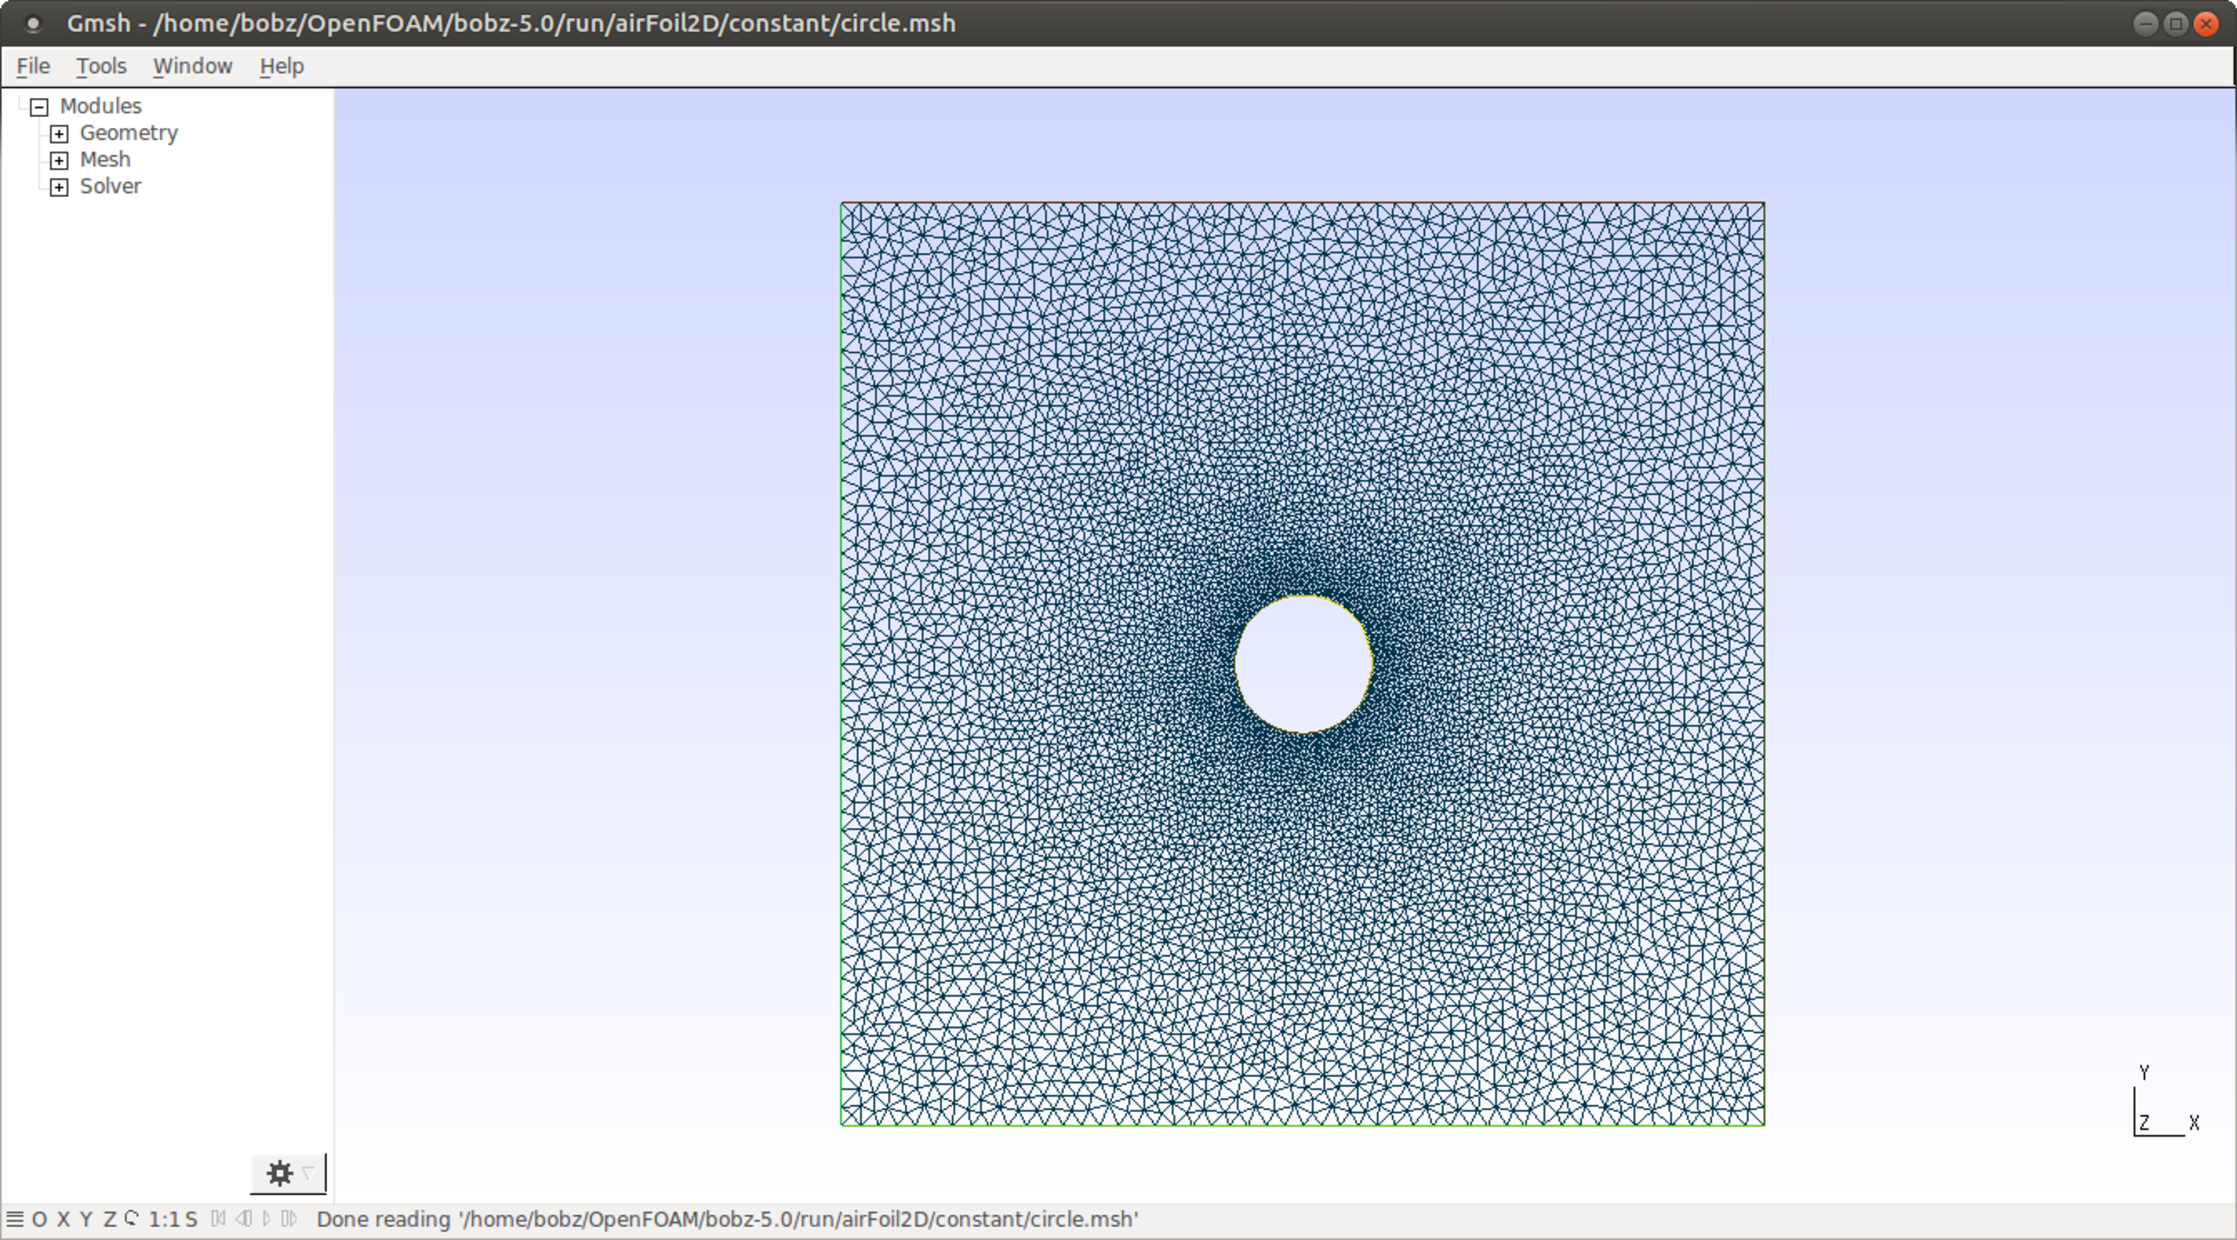
\includegraphics[width=\textwidth]{./images/malla1.pdf}
	\caption{Visió Frontal malla}
	\label{malla1}
\end{figure}
\begin{figure}[H]
	\centering
	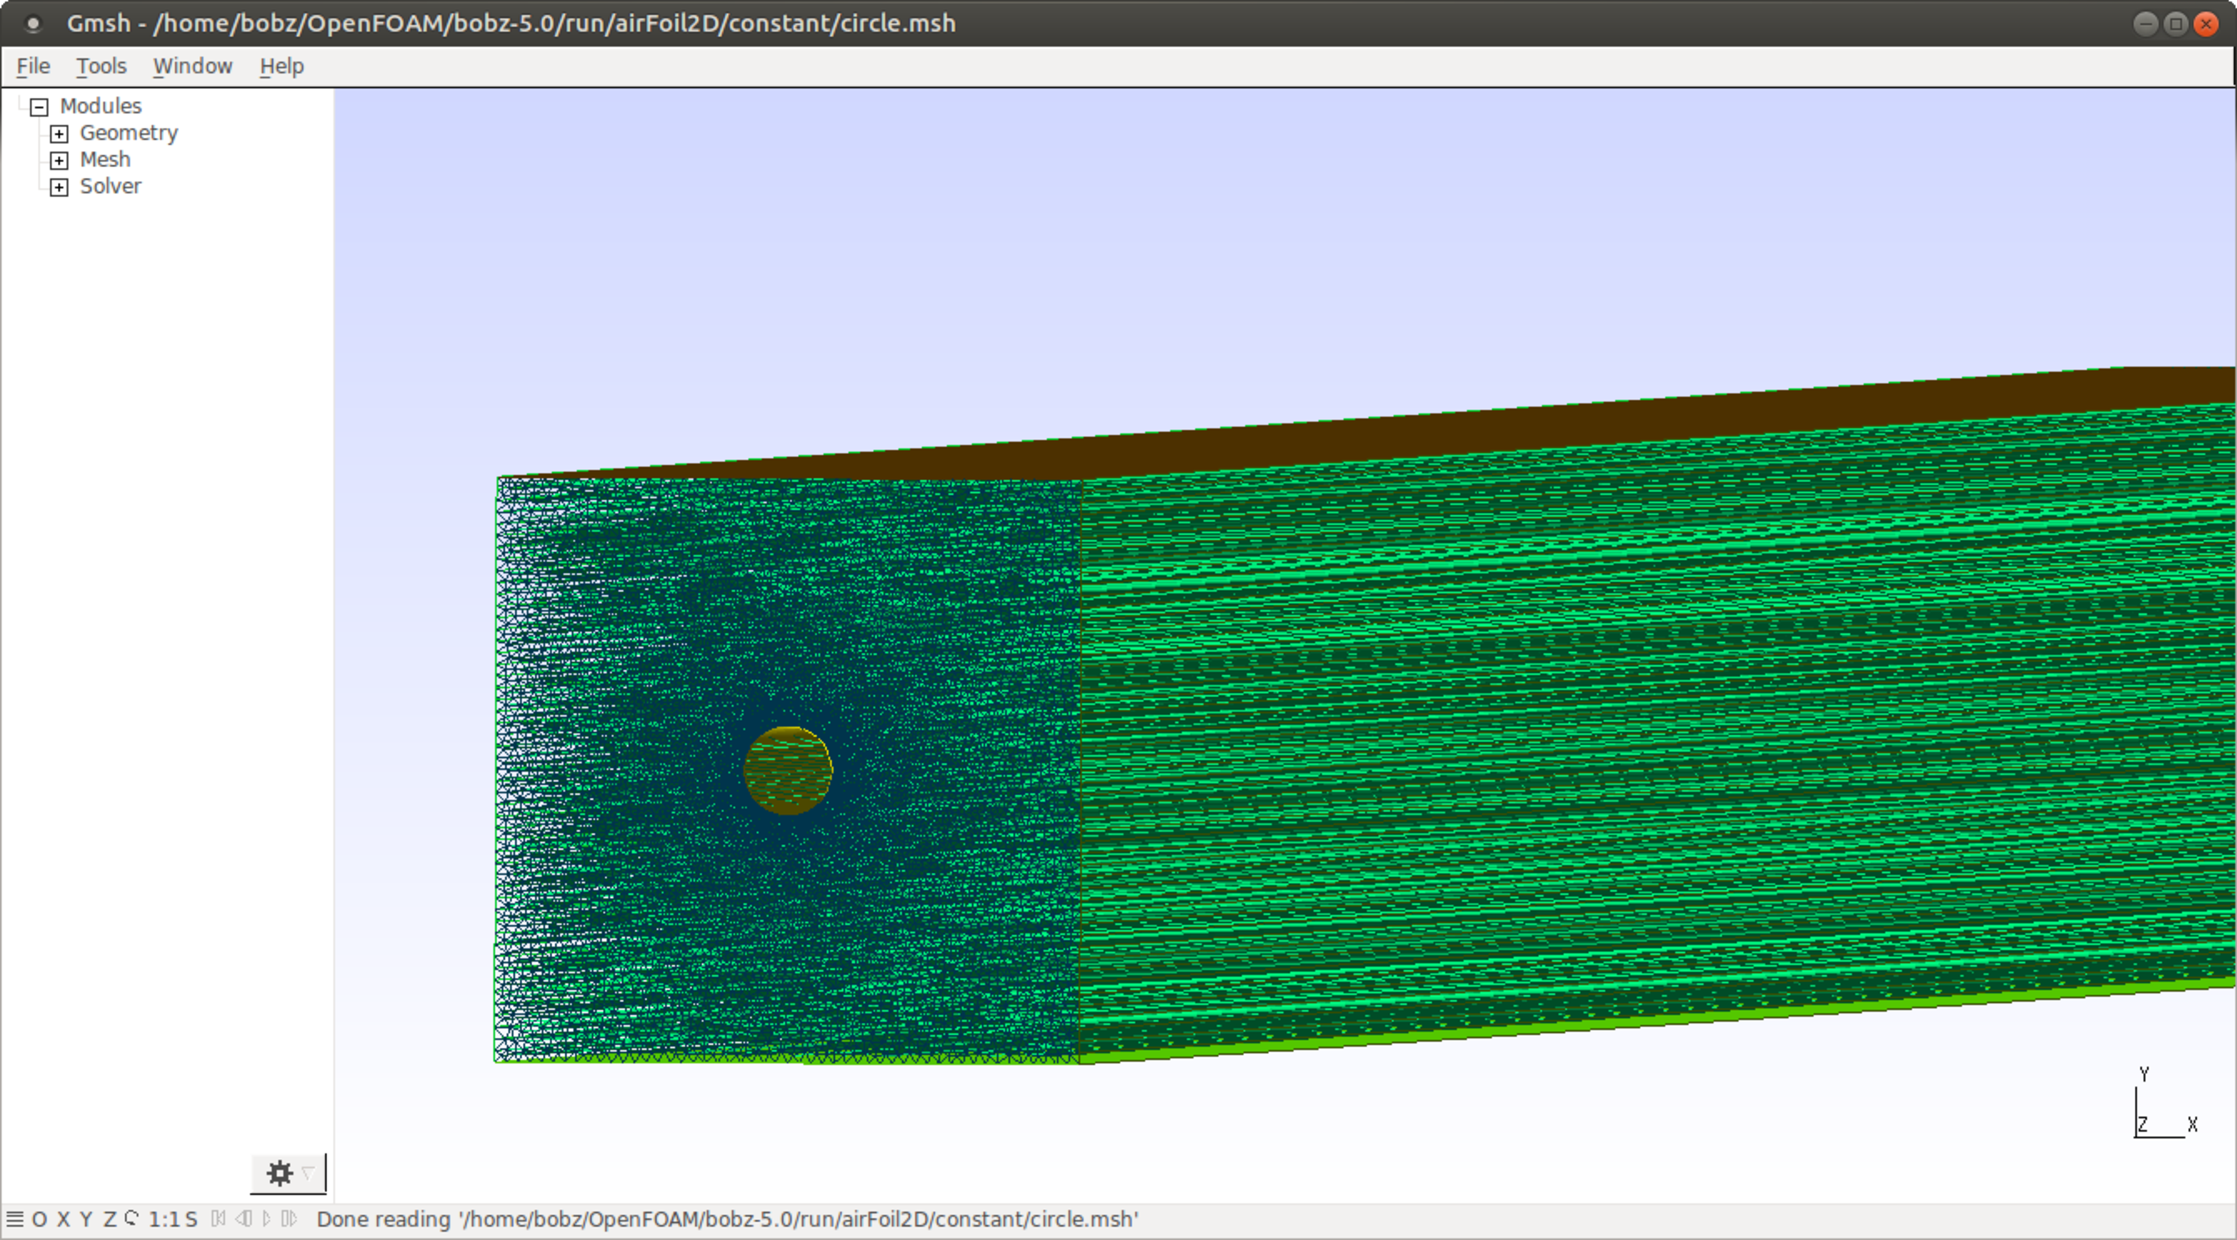
\includegraphics[width=\textwidth]{./images/malla2.pdf}
	\caption{Visió de la malla en perspectiva}
	\label{malla2}
\end{figure}
El forat cilíndric dins del volum de control representa l'antena, i així s'ha especificat a OpenFoam.